\documentclass[1p]{elsarticle_modified}
%\bibliographystyle{elsarticle-num}

%\usepackage[colorlinks]{hyperref}
%\usepackage{abbrmath_seonhwa} %\Abb, \Ascr, \Acal ,\Abf, \Afrak
\usepackage{amsfonts}
\usepackage{amssymb}
\usepackage{amsmath}
\usepackage{amsthm}
\usepackage{scalefnt}
\usepackage{amsbsy}
\usepackage{kotex}
\usepackage{caption}
\usepackage{subfig}
\usepackage{color}
\usepackage{graphicx}
\usepackage{xcolor} %% white, black, red, green, blue, cyan, magenta, yellow
\usepackage{float}
\usepackage{setspace}
\usepackage{hyperref}

\usepackage{tikz}
\usetikzlibrary{arrows}

\usepackage{multirow}
\usepackage{array} % fixed length table
\usepackage{hhline}

%%%%%%%%%%%%%%%%%%%%%
\makeatletter
\renewcommand*\env@matrix[1][\arraystretch]{%
	\edef\arraystretch{#1}%
	\hskip -\arraycolsep
	\let\@ifnextchar\new@ifnextchar
	\array{*\c@MaxMatrixCols c}}
\makeatother %https://tex.stackexchange.com/questions/14071/how-can-i-increase-the-line-spacing-in-a-matrix
%%%%%%%%%%%%%%%

\usepackage[normalem]{ulem}

\newcommand{\msout}[1]{\ifmmode\text{\sout{\ensuremath{#1}}}\else\sout{#1}\fi}
%SOURCE: \msout is \stkout macro in https://tex.stackexchange.com/questions/20609/strikeout-in-math-mode

\newcommand{\cancel}[1]{
	\ifmmode
	{\color{red}\msout{#1}}
	\else
	{\color{red}\sout{#1}}
	\fi
}

\newcommand{\add}[1]{
	{\color{blue}\uwave{#1}}
}

\newcommand{\replace}[2]{
	\ifmmode
	{\color{red}\msout{#1}}{\color{blue}\uwave{#2}}
	\else
	{\color{red}\sout{#1}}{\color{blue}\uwave{#2}}
	\fi
}

\newcommand{\Sol}{\mathcal{S}} %segment
\newcommand{\D}{D} %diagram
\newcommand{\A}{\mathcal{A}} %arc


%%%%%%%%%%%%%%%%%%%%%%%%%%%%%5 test

\def\sl{\operatorname{\textup{SL}}(2,\Cbb)}
\def\psl{\operatorname{\textup{PSL}}(2,\Cbb)}
\def\quan{\mkern 1mu \triangleright \mkern 1mu}

\theoremstyle{definition}
\newtheorem{thm}{Theorem}[section]
\newtheorem{prop}[thm]{Proposition}
\newtheorem{lem}[thm]{Lemma}
\newtheorem{ques}[thm]{Question}
\newtheorem{cor}[thm]{Corollary}
\newtheorem{defn}[thm]{Definition}
\newtheorem{exam}[thm]{Example}
\newtheorem{rmk}[thm]{Remark}
\newtheorem{alg}[thm]{Algorithm}

\newcommand{\I}{\sqrt{-1}}
\begin{document}

%\begin{frontmatter}
%
%\title{Boundary parabolic representations of knots up to 8 crossings}
%
%%% Group authors per affiliation:
%\author{Yunhi Cho} 
%\address{Department of Mathematics, University of Seoul, Seoul, Korea}
%\ead{yhcho@uos.ac.kr}
%
%
%\author{Seonhwa Kim} %\fnref{s_kim}}
%\address{Center for Geometry and Physics, Institute for Basic Science, Pohang, 37673, Korea}
%\ead{ryeona17@ibs.re.kr}
%
%\author{Hyuk Kim}
%\address{Department of Mathematical Sciences, Seoul National University, Seoul 08826, Korea}
%\ead{hyukkim@snu.ac.kr}
%
%\author{Seokbeom Yoon}
%\address{Department of Mathematical Sciences, Seoul National University, Seoul, 08826,  Korea}
%\ead{sbyoon15@snu.ac.kr}
%
%\begin{abstract}
%We find all boundary parabolic representation of knots up to 8 crossings.
%
%\end{abstract}
%\begin{keyword}
%    \MSC[2010] 57M25 
%\end{keyword}
%
%\end{frontmatter}

%\linenumbers
%\tableofcontents
%
\newcommand\colored[1]{\textcolor{white}{\rule[-0.35ex]{0.8em}{1.4ex}}\kern-0.8em\color{red} #1}%
%\newcommand\colored[1]{\textcolor{white}{ #1}\kern-2.17ex	\textcolor{white}{ #1}\kern-1.81ex	\textcolor{white}{ #1}\kern-2.15ex\color{red}#1	}

{\Large $\underline{12a_{0007}~(K12a_{0007})}$}

\setlength{\tabcolsep}{10pt}
\renewcommand{\arraystretch}{1.6}
\vspace{1cm}\begin{tabular}{m{100pt}>{\centering\arraybackslash}m{274pt}}
\multirow{5}{120pt}{
	\centering
	\includegraphics[width=112pt]{../../../GIT/diagram.site/Diagrams/png/808_12a_0007.png}\\
\ \ \ A knot diagram\footnotemark}&
\allowdisplaybreaks
\textbf{Linearized knot diagam} \\
\cline{2-2}
 &
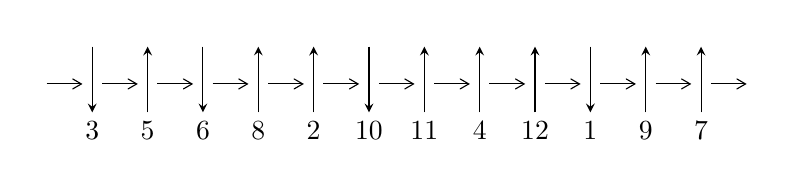
\begin{tikzpicture}[x=20pt, y=17pt]
	% nodes
	\node (C0) at (0, 0) {};
	\node (C1) at (1, 0) {};
	\node (C1U) at (1, +1) {};
	\node (C1D) at (1, -1) {3};

	\node (C2) at (2, 0) {};
	\node (C2U) at (2, +1) {};
	\node (C2D) at (2, -1) {5};

	\node (C3) at (3, 0) {};
	\node (C3U) at (3, +1) {};
	\node (C3D) at (3, -1) {6};

	\node (C4) at (4, 0) {};
	\node (C4U) at (4, +1) {};
	\node (C4D) at (4, -1) {8};

	\node (C5) at (5, 0) {};
	\node (C5U) at (5, +1) {};
	\node (C5D) at (5, -1) {2};

	\node (C6) at (6, 0) {};
	\node (C6U) at (6, +1) {};
	\node (C6D) at (6, -1) {10};

	\node (C7) at (7, 0) {};
	\node (C7U) at (7, +1) {};
	\node (C7D) at (7, -1) {11};

	\node (C8) at (8, 0) {};
	\node (C8U) at (8, +1) {};
	\node (C8D) at (8, -1) {4};

	\node (C9) at (9, 0) {};
	\node (C9U) at (9, +1) {};
	\node (C9D) at (9, -1) {12};

	\node (C10) at (10, 0) {};
	\node (C10U) at (10, +1) {};
	\node (C10D) at (10, -1) {1};

	\node (C11) at (11, 0) {};
	\node (C11U) at (11, +1) {};
	\node (C11D) at (11, -1) {9};

	\node (C12) at (12, 0) {};
	\node (C12U) at (12, +1) {};
	\node (C12D) at (12, -1) {7};
	\node (C13) at (13, 0) {};

	% arrows
	\draw[->,>={angle 60}]
	(C0) edge (C1) (C1) edge (C2) (C2) edge (C3) (C3) edge (C4) (C4) edge (C5) (C5) edge (C6) (C6) edge (C7) (C7) edge (C8) (C8) edge (C9) (C9) edge (C10) (C10) edge (C11) (C11) edge (C12) (C12) edge (C13) ;	\draw[->,>=stealth]
	(C1U) edge (C1D) (C2D) edge (C2U) (C3U) edge (C3D) (C4D) edge (C4U) (C5D) edge (C5U) (C6U) edge (C6D) (C7D) edge (C7U) (C8D) edge (C8U) (C9D) edge (C9U) (C10U) edge (C10D) (C11D) edge (C11U) (C12D) edge (C12U) ;
	\end{tikzpicture} \\
\hhline{~~} \\& 
\textbf{Solving Sequence} \\ \cline{2-2} 
 &
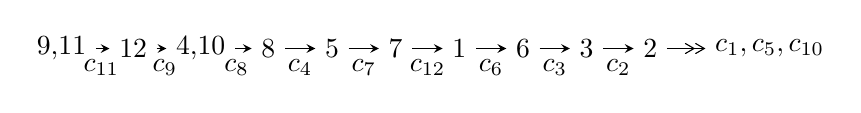
\begin{tikzpicture}[x=23pt, y=7pt]
	% node
	\node (A0) at (-1/8, 0) {9,11};
	\node (A1) at (1, 0) {12};
	\node (A2) at (33/16, 0) {4,10};
	\node (A3) at (25/8, 0) {8};
	\node (A4) at (33/8, 0) {5};
	\node (A5) at (41/8, 0) {7};
	\node (A6) at (49/8, 0) {1};
	\node (A7) at (57/8, 0) {6};
	\node (A8) at (65/8, 0) {3};
	\node (A9) at (73/8, 0) {2};
	\node (C1) at (1/2, -1) {$c_{11}$};
	\node (C2) at (3/2, -1) {$c_{9}$};
	\node (C3) at (21/8, -1) {$c_{8}$};
	\node (C4) at (29/8, -1) {$c_{4}$};
	\node (C5) at (37/8, -1) {$c_{7}$};
	\node (C6) at (45/8, -1) {$c_{12}$};
	\node (C7) at (53/8, -1) {$c_{6}$};
	\node (C8) at (61/8, -1) {$c_{3}$};
	\node (C9) at (69/8, -1) {$c_{2}$};
	\node (A10) at (11, 0) {$c_{1},c_{5},c_{10}$};

	% edge
	\draw[->,>=stealth]	
	(A0) edge (A1) (A1) edge (A2) (A2) edge (A3) (A3) edge (A4) (A4) edge (A5) (A5) edge (A6) (A6) edge (A7) (A7) edge (A8) (A8) edge (A9) ;
	\draw[->>,>={angle 60}]	
	(A9) edge (A10);
\end{tikzpicture} \\ 

\end{tabular} \\

\footnotetext{
The image of knot diagram is generated by the software ``\textbf{Draw programme}" developed by Andrew Bartholomew(\url{http://www.layer8.co.uk/maths/draw/index.htm\#Running-draw}), where we modified some parts for our purpose(\url{https://github.com/CATsTAILs/LinksPainter}).
}\phantom \\ \newline 
\centering \textbf{Ideals for irreducible components\footnotemark of $X_{\text{par}}$} 
 
\begin{align*}
I^u_{1}&=\langle 
3.08638\times10^{606} u^{134}-6.53711\times10^{606} u^{133}+\cdots+2.81019\times10^{607} b-1.77254\times10^{608},\\
\phantom{I^u_{1}}&\phantom{= \langle  }1.92887\times10^{608} u^{134}+5.80661\times10^{608} u^{133}+\cdots+1.40510\times10^{607} a+7.83298\times10^{608},\\
\phantom{I^u_{1}}&\phantom{= \langle  }u^{135}+3 u^{134}+\cdots+23 u-1\rangle \\
I^u_{2}&=\langle 
- u^4 b- u^3 b+2 u^4+u^2 b+4 u^3+b^2- b- u+2,\;a,\;u^5+u^4-2 u^3- u^2+u-1\rangle \\
\\
\end{align*}
\raggedright * 2 irreducible components of $\dim_{\mathbb{C}}=0$, with total 145 representations.\\
\footnotetext{All coefficients of polynomials are rational numbers. But the coefficients are sometimes approximated in decimal forms when there is not enough margin.}
\newpage
\renewcommand{\arraystretch}{1}
\centering \section*{I. $I^u_{1}= \langle 3.09\times10^{606} u^{134}-6.54\times10^{606} u^{133}+\cdots+2.81\times10^{607} b-1.77\times10^{608},\;1.93\times10^{608} u^{134}+5.81\times10^{608} u^{133}+\cdots+1.41\times10^{607} a+7.83\times10^{608},\;u^{135}+3 u^{134}+\cdots+23 u-1 \rangle$}
\flushleft \textbf{(i) Arc colorings}\\
\begin{tabular}{m{7pt} m{180pt} m{7pt} m{180pt} }
\flushright $a_{9}=$&$\begin{pmatrix}0\\u\end{pmatrix}$ \\
\flushright $a_{11}=$&$\begin{pmatrix}1\\0\end{pmatrix}$ \\
\flushright $a_{12}=$&$\begin{pmatrix}1\\- u^2\end{pmatrix}$ \\
\flushright $a_{4}=$&$\begin{pmatrix}-13.7277 u^{134}-41.3254 u^{133}+\cdots+1183.14 u-55.7469\\-0.109828 u^{134}+0.232621 u^{133}+\cdots-105.020 u+6.30755\end{pmatrix}$ \\
\flushright $a_{10}=$&$\begin{pmatrix}u\\- u^3+u\end{pmatrix}$ \\
\flushright $a_{8}=$&$\begin{pmatrix}10.5104 u^{134}+28.1213 u^{133}+\cdots-1273.21 u+77.3616\\5.06292 u^{134}+13.4726 u^{133}+\cdots+44.0782 u-4.59033\end{pmatrix}$ \\
\flushright $a_{5}=$&$\begin{pmatrix}-13.0648 u^{134}-34.5807 u^{133}+\cdots+1060.19 u-61.4604\\-3.59206 u^{134}-9.85582 u^{133}+\cdots+61.8222 u-1.81266\end{pmatrix}$ \\
\flushright $a_{7}=$&$\begin{pmatrix}5.44751 u^{134}+14.6486 u^{133}+\cdots-1317.28 u+81.9520\\5.06292 u^{134}+13.4726 u^{133}+\cdots+44.0782 u-4.59033\end{pmatrix}$ \\
\flushright $a_{1}=$&$\begin{pmatrix}-5.24791 u^{134}-8.31601 u^{133}+\cdots-654.297 u+37.1633\\1.85841 u^{134}+4.39282 u^{133}+\cdots+18.2202 u-2.17981\end{pmatrix}$ \\
\flushright $a_{6}=$&$\begin{pmatrix}10.4058 u^{134}+26.7954 u^{133}+\cdots-1291.76 u+80.7778\\4.74187 u^{134}+13.2057 u^{133}+\cdots+1.89833 u-3.03646\end{pmatrix}$ \\
\flushright $a_{3}=$&$\begin{pmatrix}-5.13933 u^{134}-9.01892 u^{133}+\cdots-9.48553 u-6.83756\\-2.44953 u^{134}-7.38833 u^{133}+\cdots+199.596 u-10.1484\end{pmatrix}$ \\
\flushright $a_{2}=$&$\begin{pmatrix}5.18030 u^{134}+17.5516 u^{133}+\cdots-757.386 u+41.6323\\-0.304850 u^{134}-2.35761 u^{133}+\cdots+245.506 u-12.4320\end{pmatrix}$\\&\end{tabular}
\flushleft \textbf{(ii) Obstruction class $= -1$}\\~\\
\flushleft \textbf{(iii) Cusp Shapes $= -9.36282 u^{134}-20.3123 u^{133}+\cdots-666.463 u+49.0376$}\\~\\
\newpage\renewcommand{\arraystretch}{1}
\flushleft \textbf{(iv) u-Polynomials at the component}\newline \\
\begin{tabular}{m{50pt}|m{274pt}}
Crossings & \hspace{64pt}u-Polynomials at each crossing \\
\hline $$\begin{aligned}c_{1}\end{aligned}$$&$\begin{aligned}
&u^{135}+64 u^{134}+\cdots+158 u-1
\end{aligned}$\\
\hline $$\begin{aligned}c_{2},c_{5}\end{aligned}$$&$\begin{aligned}
&u^{135}+6 u^{134}+\cdots-2 u-1
\end{aligned}$\\
\hline $$\begin{aligned}c_{3}\end{aligned}$$&$\begin{aligned}
&u^{135}-6 u^{134}+\cdots+18532724 u-1174793
\end{aligned}$\\
\hline $$\begin{aligned}c_{4},c_{8}\end{aligned}$$&$\begin{aligned}
&u^{135}- u^{134}+\cdots+5120 u-1024
\end{aligned}$\\
\hline $$\begin{aligned}c_{6}\end{aligned}$$&$\begin{aligned}
&u^{135}+3 u^{134}+\cdots+12401 u-47809
\end{aligned}$\\
\hline $$\begin{aligned}c_{7}\end{aligned}$$&$\begin{aligned}
&u^{135}-3 u^{134}+\cdots+17948537 u-2522669
\end{aligned}$\\
\hline $$\begin{aligned}c_{9},c_{11}\end{aligned}$$&$\begin{aligned}
&u^{135}+3 u^{134}+\cdots+23 u-1
\end{aligned}$\\
\hline $$\begin{aligned}c_{10}\end{aligned}$$&$\begin{aligned}
&u^{135}-23 u^{134}+\cdots+3 u-1
\end{aligned}$\\
\hline $$\begin{aligned}c_{12}\end{aligned}$$&$\begin{aligned}
&u^{135}+9 u^{134}+\cdots+3 u+1
\end{aligned}$\\
\hline
\end{tabular}\\~\\
\newpage\renewcommand{\arraystretch}{1}
\flushleft \textbf{(v) Riley Polynomials at the component}\newline \\
\begin{tabular}{m{50pt}|m{274pt}}
Crossings & \hspace{64pt}Riley Polynomials at each crossing \\
\hline $$\begin{aligned}c_{1}\end{aligned}$$&$\begin{aligned}
&y^{135}+20 y^{134}+\cdots+22410 y-1
\end{aligned}$\\
\hline $$\begin{aligned}c_{2},c_{5}\end{aligned}$$&$\begin{aligned}
&y^{135}+64 y^{134}+\cdots+158 y-1
\end{aligned}$\\
\hline $$\begin{aligned}c_{3}\end{aligned}$$&$\begin{aligned}
&y^{135}-24 y^{134}+\cdots+270394515667686 y-1380138592849
\end{aligned}$\\
\hline $$\begin{aligned}c_{4},c_{8}\end{aligned}$$&$\begin{aligned}
&y^{135}+55 y^{134}+\cdots-24117248 y-1048576
\end{aligned}$\\
\hline $$\begin{aligned}c_{6}\end{aligned}$$&$\begin{aligned}
&y^{135}+149 y^{134}+\cdots-218902272299 y-2285700481
\end{aligned}$\\
\hline $$\begin{aligned}c_{7}\end{aligned}$$&$\begin{aligned}
&y^{135}+85 y^{134}+\cdots+285856654348325 y-6363858883561
\end{aligned}$\\
\hline $$\begin{aligned}c_{9},c_{11}\end{aligned}$$&$\begin{aligned}
&y^{135}-95 y^{134}+\cdots-23 y-1
\end{aligned}$\\
\hline $$\begin{aligned}c_{10}\end{aligned}$$&$\begin{aligned}
&y^{135}+9 y^{134}+\cdots-23 y-1
\end{aligned}$\\
\hline $$\begin{aligned}c_{12}\end{aligned}$$&$\begin{aligned}
&y^{135}-23 y^{134}+\cdots+9 y-1
\end{aligned}$\\
\hline
\end{tabular}\\~\\
\newpage\flushleft \textbf{(vi) Complex Volumes and Cusp Shapes}
$$\begin{array}{c|c|c}  
\text{Solutions to }I^u_{1}& \I (\text{vol} + \sqrt{-1}CS) & \text{Cusp shape}\\
 \hline 
\begin{aligned}
u &= -0.568524 + 0.805822 I \\
a &= -1.186920 + 0.557168 I \\
b &= -1.55948 + 0.08612 I\end{aligned}
 & -7.52069 - 3.51563 I & \phantom{-0.000000 } 0 \\ \hline\begin{aligned}
u &= -0.568524 - 0.805822 I \\
a &= -1.186920 - 0.557168 I \\
b &= -1.55948 - 0.08612 I\end{aligned}
 & -7.52069 + 3.51563 I & \phantom{-0.000000 } 0 \\ \hline\begin{aligned}
u &= -0.907886 + 0.454916 I \\
a &= \phantom{-}0.68514 - 1.26035 I \\
b &= \phantom{-}0.880008 + 0.743585 I\end{aligned}
 & -6.41600 - 1.19724 I & \phantom{-0.000000 } 0 \\ \hline\begin{aligned}
u &= -0.907886 - 0.454916 I \\
a &= \phantom{-}0.68514 + 1.26035 I \\
b &= \phantom{-}0.880008 - 0.743585 I\end{aligned}
 & -6.41600 + 1.19724 I & \phantom{-0.000000 } 0 \\ \hline\begin{aligned}
u &= -1.007480 + 0.177190 I \\
a &= \phantom{-}1.317070 + 0.096501 I \\
b &= \phantom{-}0.423505 + 0.082153 I\end{aligned}
 & \phantom{-}0.05421 - 4.55763 I & \phantom{-0.000000 } 0 \\ \hline\begin{aligned}
u &= -1.007480 - 0.177190 I \\
a &= \phantom{-}1.317070 - 0.096501 I \\
b &= \phantom{-}0.423505 - 0.082153 I\end{aligned}
 & \phantom{-}0.05421 + 4.55763 I & \phantom{-0.000000 } 0 \\ \hline\begin{aligned}
u &= \phantom{-}1.026060 + 0.044609 I \\
a &= -0.688975 + 0.420532 I \\
b &= -2.76943 + 3.04188 I\end{aligned}
 & \phantom{-}1.53614 + 3.00834 I & \phantom{-0.000000 } 0 \\ \hline\begin{aligned}
u &= \phantom{-}1.026060 - 0.044609 I \\
a &= -0.688975 - 0.420532 I \\
b &= -2.76943 - 3.04188 I\end{aligned}
 & \phantom{-}1.53614 - 3.00834 I & \phantom{-0.000000 } 0 \\ \hline\begin{aligned}
u &= \phantom{-}0.116944 + 1.020390 I \\
a &= \phantom{-}0.391000 + 0.849314 I \\
b &= \phantom{-}0.775161 - 0.064942 I\end{aligned}
 & \phantom{-}1.03911 + 2.79672 I & \phantom{-0.000000 } 0 \\ \hline\begin{aligned}
u &= \phantom{-}0.116944 - 1.020390 I \\
a &= \phantom{-}0.391000 - 0.849314 I \\
b &= \phantom{-}0.775161 + 0.064942 I\end{aligned}
 & \phantom{-}1.03911 - 2.79672 I & \phantom{-0.000000 } 0\\
 \hline 
 \end{array}$$\newpage$$\begin{array}{c|c|c}  
\text{Solutions to }I^u_{1}& \I (\text{vol} + \sqrt{-1}CS) & \text{Cusp shape}\\
 \hline 
\begin{aligned}
u &= -0.419714 + 0.963008 I \\
a &= -1.113320 + 0.500212 I \\
b &= -1.64463 + 0.09604 I\end{aligned}
 & -7.94598 + 4.71009 I & \phantom{-0.000000 } 0 \\ \hline\begin{aligned}
u &= -0.419714 - 0.963008 I \\
a &= -1.113320 - 0.500212 I \\
b &= -1.64463 - 0.09604 I\end{aligned}
 & -7.94598 - 4.71009 I & \phantom{-0.000000 } 0 \\ \hline\begin{aligned}
u &= \phantom{-}1.051520 + 0.006262 I \\
a &= \phantom{-}0.564038 + 0.595897 I \\
b &= \phantom{-}3.87487 + 1.91741 I\end{aligned}
 & \phantom{-}2.86400 + 1.41798 I & \phantom{-0.000000 } 0 \\ \hline\begin{aligned}
u &= \phantom{-}1.051520 - 0.006262 I \\
a &= \phantom{-}0.564038 - 0.595897 I \\
b &= \phantom{-}3.87487 - 1.91741 I\end{aligned}
 & \phantom{-}2.86400 - 1.41798 I & \phantom{-0.000000 } 0 \\ \hline\begin{aligned}
u &= \phantom{-}1.043770 + 0.152675 I \\
a &= -0.464877 - 0.956012 I \\
b &= -2.93917 - 0.27243 I\end{aligned}
 & -2.46009 + 0.50056 I & \phantom{-0.000000 } 0 \\ \hline\begin{aligned}
u &= \phantom{-}1.043770 - 0.152675 I \\
a &= -0.464877 + 0.956012 I \\
b &= -2.93917 + 0.27243 I\end{aligned}
 & -2.46009 - 0.50056 I & \phantom{-0.000000 } 0 \\ \hline\begin{aligned}
u &= \phantom{-}0.083016 + 1.051850 I \\
a &= -0.870439 + 0.409276 I \\
b &= -1.83729 - 0.09226 I\end{aligned}
 & \phantom{-}0.83592 + 5.69951 I & \phantom{-0.000000 } 0 \\ \hline\begin{aligned}
u &= \phantom{-}0.083016 - 1.051850 I \\
a &= -0.870439 - 0.409276 I \\
b &= -1.83729 + 0.09226 I\end{aligned}
 & \phantom{-}0.83592 - 5.69951 I & \phantom{-0.000000 } 0 \\ \hline\begin{aligned}
u &= -1.021600 + 0.270915 I \\
a &= \phantom{-}0.998429 - 0.892064 I \\
b &= \phantom{-}1.221320 + 0.406339 I\end{aligned}
 & -2.95130 - 3.55729 I & \phantom{-0.000000 } 0 \\ \hline\begin{aligned}
u &= -1.021600 - 0.270915 I \\
a &= \phantom{-}0.998429 + 0.892064 I \\
b &= \phantom{-}1.221320 - 0.406339 I\end{aligned}
 & -2.95130 + 3.55729 I & \phantom{-0.000000 } 0\\
 \hline 
 \end{array}$$\newpage$$\begin{array}{c|c|c}  
\text{Solutions to }I^u_{1}& \I (\text{vol} + \sqrt{-1}CS) & \text{Cusp shape}\\
 \hline 
\begin{aligned}
u &= -1.055660 + 0.106193 I \\
a &= \phantom{-}1.077190 + 0.842689 I \\
b &= \phantom{-}0.517475 + 0.017390 I\end{aligned}
 & \phantom{-}1.92024 - 4.49255 I & \phantom{-0.000000 } 0 \\ \hline\begin{aligned}
u &= -1.055660 - 0.106193 I \\
a &= \phantom{-}1.077190 - 0.842689 I \\
b &= \phantom{-}0.517475 - 0.017390 I\end{aligned}
 & \phantom{-}1.92024 + 4.49255 I & \phantom{-0.000000 } 0 \\ \hline\begin{aligned}
u &= \phantom{-}0.080608 + 0.921052 I \\
a &= \phantom{-}0.873120 - 0.320604 I \\
b &= \phantom{-}1.97968 + 0.02512 I\end{aligned}
 & \phantom{-}0.007085 + 0.583291 I & \phantom{-0.000000 } 0 \\ \hline\begin{aligned}
u &= \phantom{-}0.080608 - 0.921052 I \\
a &= \phantom{-}0.873120 + 0.320604 I \\
b &= \phantom{-}1.97968 - 0.02512 I\end{aligned}
 & \phantom{-}0.007085 - 0.583291 I & \phantom{-0.000000 } 0 \\ \hline\begin{aligned}
u &= -1.085860 + 0.069941 I \\
a &= \phantom{-}0.275746 + 1.215720 I \\
b &= \phantom{-}0.321621 - 1.157430 I\end{aligned}
 & \phantom{-}3.24444 - 3.62921 I & \phantom{-0.000000 } 0 \\ \hline\begin{aligned}
u &= -1.085860 - 0.069941 I \\
a &= \phantom{-}0.275746 - 1.215720 I \\
b &= \phantom{-}0.321621 + 1.157430 I\end{aligned}
 & \phantom{-}3.24444 + 3.62921 I & \phantom{-0.000000 } 0 \\ \hline\begin{aligned}
u &= \phantom{-}1.089220 + 0.056094 I \\
a &= \phantom{-}0.086119 + 0.368937 I \\
b &= \phantom{-}0.55341 - 6.16169 I\end{aligned}
 & \phantom{-}2.17840 + 2.18123 I & \phantom{-0.000000 } 0 \\ \hline\begin{aligned}
u &= \phantom{-}1.089220 - 0.056094 I \\
a &= \phantom{-}0.086119 - 0.368937 I \\
b &= \phantom{-}0.55341 + 6.16169 I\end{aligned}
 & \phantom{-}2.17840 - 2.18123 I & \phantom{-0.000000 } 0 \\ \hline\begin{aligned}
u &= \phantom{-}0.009853 + 1.093610 I \\
a &= -0.435161 - 0.909331 I \\
b &= -0.811741 + 0.004845 I\end{aligned}
 & -1.01744 + 7.35867 I & \phantom{-0.000000 } 0 \\ \hline\begin{aligned}
u &= \phantom{-}0.009853 - 1.093610 I \\
a &= -0.435161 + 0.909331 I \\
b &= -0.811741 - 0.004845 I\end{aligned}
 & -1.01744 - 7.35867 I & \phantom{-0.000000 } 0\\
 \hline 
 \end{array}$$\newpage$$\begin{array}{c|c|c}  
\text{Solutions to }I^u_{1}& \I (\text{vol} + \sqrt{-1}CS) & \text{Cusp shape}\\
 \hline 
\begin{aligned}
u &= -0.416447 + 0.803539 I \\
a &= \phantom{-}1.191210 - 0.476871 I \\
b &= \phantom{-}1.59991 - 0.15322 I\end{aligned}
 & -4.35305 + 0.80319 I & \phantom{-0.000000 } 0 \\ \hline\begin{aligned}
u &= -0.416447 - 0.803539 I \\
a &= \phantom{-}1.191210 + 0.476871 I \\
b &= \phantom{-}1.59991 + 0.15322 I\end{aligned}
 & -4.35305 - 0.80319 I & \phantom{-0.000000 } 0 \\ \hline\begin{aligned}
u &= \phantom{-}1.040580 + 0.349191 I \\
a &= \phantom{-}0.446852 - 0.394829 I \\
b &= \phantom{-}0.190132 + 1.142410 I\end{aligned}
 & \phantom{-}1.54023 - 0.58667 I & \phantom{-0.000000 } 0 \\ \hline\begin{aligned}
u &= \phantom{-}1.040580 - 0.349191 I \\
a &= \phantom{-}0.446852 + 0.394829 I \\
b &= \phantom{-}0.190132 - 1.142410 I\end{aligned}
 & \phantom{-}1.54023 + 0.58667 I & \phantom{-0.000000 } 0 \\ \hline\begin{aligned}
u &= \phantom{-}0.438285 + 1.007090 I \\
a &= \phantom{-}0.454121 + 0.675347 I \\
b &= \phantom{-}0.821512 - 0.305548 I\end{aligned}
 & \phantom{-}1.20916 + 1.59276 I & \phantom{-0.000000 } 0 \\ \hline\begin{aligned}
u &= \phantom{-}0.438285 - 1.007090 I \\
a &= \phantom{-}0.454121 - 0.675347 I \\
b &= \phantom{-}0.821512 + 0.305548 I\end{aligned}
 & \phantom{-}1.20916 - 1.59276 I & \phantom{-0.000000 } 0 \\ \hline\begin{aligned}
u &= -1.097860 + 0.038828 I \\
a &= -0.637062 + 1.120900 I \\
b &= -0.771440 - 0.894856 I\end{aligned}
 & \phantom{-}4.13066 - 2.35961 I & \phantom{-0.000000 } 0 \\ \hline\begin{aligned}
u &= -1.097860 - 0.038828 I \\
a &= -0.637062 - 1.120900 I \\
b &= -0.771440 + 0.894856 I\end{aligned}
 & \phantom{-}4.13066 + 2.35961 I & \phantom{-0.000000 } 0 \\ \hline\begin{aligned}
u &= \phantom{-}1.096500 + 0.092685 I \\
a &= \phantom{-}0.573386 + 0.848744 I \\
b &= \phantom{-}3.09848 + 0.80652 I\end{aligned}
 & \phantom{-}1.79298 + 3.12616 I & \phantom{-0.000000 } 0 \\ \hline\begin{aligned}
u &= \phantom{-}1.096500 - 0.092685 I \\
a &= \phantom{-}0.573386 - 0.848744 I \\
b &= \phantom{-}3.09848 - 0.80652 I\end{aligned}
 & \phantom{-}1.79298 - 3.12616 I & \phantom{-0.000000 } 0\\
 \hline 
 \end{array}$$\newpage$$\begin{array}{c|c|c}  
\text{Solutions to }I^u_{1}& \I (\text{vol} + \sqrt{-1}CS) & \text{Cusp shape}\\
 \hline 
\begin{aligned}
u &= -1.111950 + 0.006804 I \\
a &= -1.126920 + 0.487485 I \\
b &= -0.423626 - 0.004236 I\end{aligned}
 & \phantom{-}4.49122 - 0.85357 I & \phantom{-0.000000 } 0 \\ \hline\begin{aligned}
u &= -1.111950 - 0.006804 I \\
a &= -1.126920 - 0.487485 I \\
b &= -0.423626 + 0.004236 I\end{aligned}
 & \phantom{-}4.49122 + 0.85357 I & \phantom{-0.000000 } 0 \\ \hline\begin{aligned}
u &= \phantom{-}0.885186 + 0.050073 I \\
a &= -0.740848 + 0.127427 I \\
b &= -0.10936 - 2.32435 I\end{aligned}
 & \phantom{-}0.92608 + 2.64149 I & \phantom{-0.000000 } 0 \\ \hline\begin{aligned}
u &= \phantom{-}0.885186 - 0.050073 I \\
a &= -0.740848 - 0.127427 I \\
b &= -0.10936 + 2.32435 I\end{aligned}
 & \phantom{-}0.92608 - 2.64149 I & \phantom{-0.000000 } 0 \\ \hline\begin{aligned}
u &= -0.118952 + 0.869942 I \\
a &= -0.328619 - 1.037610 I \\
b &= -0.719254 - 0.066072 I\end{aligned}
 & -2.45542 + 0.43451 I & \phantom{-0.000000 } 0 \\ \hline\begin{aligned}
u &= -0.118952 - 0.869942 I \\
a &= -0.328619 + 1.037610 I \\
b &= -0.719254 + 0.066072 I\end{aligned}
 & -2.45542 - 0.43451 I & \phantom{-0.000000 } 0 \\ \hline\begin{aligned}
u &= \phantom{-}1.125470 + 0.117732 I \\
a &= -0.612434 - 0.905025 I \\
b &= -2.86154 - 0.78542 I\end{aligned}
 & -0.46769 + 8.00362 I & \phantom{-0.000000 } 0 \\ \hline\begin{aligned}
u &= \phantom{-}1.125470 - 0.117732 I \\
a &= -0.612434 + 0.905025 I \\
b &= -2.86154 + 0.78542 I\end{aligned}
 & -0.46769 - 8.00362 I & \phantom{-0.000000 } 0 \\ \hline\begin{aligned}
u &= -1.040870 + 0.448369 I \\
a &= -0.587288 + 1.058760 I \\
b &= -1.02358 - 1.03227 I\end{aligned}
 & -2.40247 - 5.42914 I & \phantom{-0.000000 } 0 \\ \hline\begin{aligned}
u &= -1.040870 - 0.448369 I \\
a &= -0.587288 - 1.058760 I \\
b &= -1.02358 + 1.03227 I\end{aligned}
 & -2.40247 + 5.42914 I & \phantom{-0.000000 } 0\\
 \hline 
 \end{array}$$\newpage$$\begin{array}{c|c|c}  
\text{Solutions to }I^u_{1}& \I (\text{vol} + \sqrt{-1}CS) & \text{Cusp shape}\\
 \hline 
\begin{aligned}
u &= \phantom{-}1.15383\phantom{ +0.000000I} \\
a &= \phantom{-}0.248512\phantom{ +0.000000I} \\
b &= -0.617227\phantom{ +0.000000I}\end{aligned}
 & \phantom{-}2.30295\phantom{ +0.000000I} & \phantom{-0.000000 } 0 \\ \hline\begin{aligned}
u &= \phantom{-}0.797291 + 0.240741 I \\
a &= \phantom{-}0.152484 + 1.301610 I \\
b &= \phantom{-}1.96500 - 0.41263 I\end{aligned}
 & -3.03176 + 0.85487 I & \phantom{-0.000000 } 0 \\ \hline\begin{aligned}
u &= \phantom{-}0.797291 - 0.240741 I \\
a &= \phantom{-}0.152484 - 1.301610 I \\
b &= \phantom{-}1.96500 + 0.41263 I\end{aligned}
 & -3.03176 - 0.85487 I & \phantom{-0.000000 } 0 \\ \hline\begin{aligned}
u &= -1.159770 + 0.238949 I \\
a &= -0.866476 + 0.823520 I \\
b &= -1.34363 - 0.63804 I\end{aligned}
 & \phantom{-}2.64360 - 6.29046 I & \phantom{-0.000000 } 0 \\ \hline\begin{aligned}
u &= -1.159770 - 0.238949 I \\
a &= -0.866476 - 0.823520 I \\
b &= -1.34363 + 0.63804 I\end{aligned}
 & \phantom{-}2.64360 + 6.29046 I & \phantom{-0.000000 } 0 \\ \hline\begin{aligned}
u &= -1.067580 + 0.544991 I \\
a &= \phantom{-}0.719832 - 0.975059 I \\
b &= \phantom{-}1.25728 + 0.91896 I\end{aligned}
 & -5.87319 - 10.08940 I & \phantom{-0.000000 } 0 \\ \hline\begin{aligned}
u &= -1.067580 - 0.544991 I \\
a &= \phantom{-}0.719832 + 0.975059 I \\
b &= \phantom{-}1.25728 - 0.91896 I\end{aligned}
 & -5.87319 + 10.08940 I & \phantom{-0.000000 } 0 \\ \hline\begin{aligned}
u &= -0.087955 + 1.201330 I \\
a &= \phantom{-}0.944422 - 0.493344 I \\
b &= \phantom{-}1.70851 + 0.01513 I\end{aligned}
 & -5.66349 + 5.47096 I & \phantom{-0.000000 } 0 \\ \hline\begin{aligned}
u &= -0.087955 - 1.201330 I \\
a &= \phantom{-}0.944422 + 0.493344 I \\
b &= \phantom{-}1.70851 - 0.01513 I\end{aligned}
 & -5.66349 - 5.47096 I & \phantom{-0.000000 } 0 \\ \hline\begin{aligned}
u &= -1.188910 + 0.286559 I \\
a &= \phantom{-}0.889919 - 0.773016 I \\
b &= \phantom{-}1.44145 + 0.59362 I\end{aligned}
 & \phantom{-}0.38712 - 11.78350 I & \phantom{-0.000000 } 0\\
 \hline 
 \end{array}$$\newpage$$\begin{array}{c|c|c}  
\text{Solutions to }I^u_{1}& \I (\text{vol} + \sqrt{-1}CS) & \text{Cusp shape}\\
 \hline 
\begin{aligned}
u &= -1.188910 - 0.286559 I \\
a &= \phantom{-}0.889919 + 0.773016 I \\
b &= \phantom{-}1.44145 - 0.59362 I\end{aligned}
 & \phantom{-}0.38712 + 11.78350 I & \phantom{-0.000000 } 0 \\ \hline\begin{aligned}
u &= \phantom{-}0.019858 + 1.238580 I \\
a &= -0.897984 + 0.501763 I \\
b &= -1.69963 - 0.06811 I\end{aligned}
 & -0.80905 + 8.28455 I & \phantom{-0.000000 } 0 \\ \hline\begin{aligned}
u &= \phantom{-}0.019858 - 1.238580 I \\
a &= -0.897984 - 0.501763 I \\
b &= -1.69963 + 0.06811 I\end{aligned}
 & -0.80905 - 8.28455 I & \phantom{-0.000000 } 0 \\ \hline\begin{aligned}
u &= \phantom{-}0.569961 + 1.127270 I \\
a &= -0.531317 - 0.663723 I \\
b &= -0.973907 + 0.344786 I\end{aligned}
 & -0.79606 - 2.83608 I & \phantom{-0.000000 } 0 \\ \hline\begin{aligned}
u &= \phantom{-}0.569961 - 1.127270 I \\
a &= -0.531317 + 0.663723 I \\
b &= -0.973907 - 0.344786 I\end{aligned}
 & -0.79606 + 2.83608 I & \phantom{-0.000000 } 0 \\ \hline\begin{aligned}
u &= \phantom{-}0.820697 + 0.963046 I \\
a &= -0.551140 - 0.561218 I \\
b &= -1.062630 + 0.634441 I\end{aligned}
 & -1.95084 + 4.11866 I & \phantom{-0.000000 } 0 \\ \hline\begin{aligned}
u &= \phantom{-}0.820697 - 0.963046 I \\
a &= -0.551140 + 0.561218 I \\
b &= -1.062630 - 0.634441 I\end{aligned}
 & -1.95084 - 4.11866 I & \phantom{-0.000000 } 0 \\ \hline\begin{aligned}
u &= \phantom{-}0.562883 + 0.443226 I \\
a &= \phantom{-}0.580480 + 0.461713 I \\
b &= \phantom{-}0.027447 - 0.872637 I\end{aligned}
 & \phantom{-}0.66023 + 1.44451 I & \phantom{-0.000000 } 0 \\ \hline\begin{aligned}
u &= \phantom{-}0.562883 - 0.443226 I \\
a &= \phantom{-}0.580480 - 0.461713 I \\
b &= \phantom{-}0.027447 + 0.872637 I\end{aligned}
 & \phantom{-}0.66023 - 1.44451 I & \phantom{-0.000000 } 0 \\ \hline\begin{aligned}
u &= \phantom{-}0.008679 + 1.294510 I \\
a &= \phantom{-}0.901083 - 0.524151 I \\
b &= \phantom{-}1.67286 + 0.06156 I\end{aligned}
 & -3.15409 + 13.45310 I & \phantom{-0.000000 } 0\\
 \hline 
 \end{array}$$\newpage$$\begin{array}{c|c|c}  
\text{Solutions to }I^u_{1}& \I (\text{vol} + \sqrt{-1}CS) & \text{Cusp shape}\\
 \hline 
\begin{aligned}
u &= \phantom{-}0.008679 - 1.294510 I \\
a &= \phantom{-}0.901083 + 0.524151 I \\
b &= \phantom{-}1.67286 - 0.06156 I\end{aligned}
 & -3.15409 - 13.45310 I & \phantom{-0.000000 } 0 \\ \hline\begin{aligned}
u &= \phantom{-}0.621734 + 0.332061 I \\
a &= \phantom{-}0.11218 + 1.65942 I \\
b &= \phantom{-}1.52142 - 0.25068 I\end{aligned}
 & -1.58896 - 6.54144 I & \phantom{-0.000000 } 0 \\ \hline\begin{aligned}
u &= \phantom{-}0.621734 - 0.332061 I \\
a &= \phantom{-}0.11218 - 1.65942 I \\
b &= \phantom{-}1.52142 + 0.25068 I\end{aligned}
 & -1.58896 + 6.54144 I & \phantom{-0.000000 } 0 \\ \hline\begin{aligned}
u &= -1.259540 + 0.463280 I \\
a &= -0.697654 - 0.564354 I \\
b &= -0.284305 - 0.259378 I\end{aligned}
 & \phantom{-}1.11874 - 5.27197 I & \phantom{-0.000000 } 0 \\ \hline\begin{aligned}
u &= -1.259540 - 0.463280 I \\
a &= -0.697654 + 0.564354 I \\
b &= -0.284305 + 0.259378 I\end{aligned}
 & \phantom{-}1.11874 + 5.27197 I & \phantom{-0.000000 } 0 \\ \hline\begin{aligned}
u &= -1.359480 + 0.117427 I \\
a &= -0.490412 + 0.278971 I \\
b &= -0.235539 + 0.060510 I\end{aligned}
 & \phantom{-}6.64310 - 2.61859 I & \phantom{-0.000000 } 0 \\ \hline\begin{aligned}
u &= -1.359480 - 0.117427 I \\
a &= -0.490412 - 0.278971 I \\
b &= -0.235539 - 0.060510 I\end{aligned}
 & \phantom{-}6.64310 + 2.61859 I & \phantom{-0.000000 } 0 \\ \hline\begin{aligned}
u &= \phantom{-}0.582918 + 0.205812 I \\
a &= \phantom{-}0.17559 - 1.61087 I \\
b &= -1.40341 + 0.48169 I\end{aligned}
 & \phantom{-}0.69426 - 1.95174 I & \phantom{-0.000000 -}0. + 5.64029 I \\ \hline\begin{aligned}
u &= \phantom{-}0.582918 - 0.205812 I \\
a &= \phantom{-}0.17559 + 1.61087 I \\
b &= -1.40341 - 0.48169 I\end{aligned}
 & \phantom{-}0.69426 + 1.95174 I & \phantom{-0.000000 } 0. - 5.64029 I \\ \hline\begin{aligned}
u &= -1.327410 + 0.462550 I \\
a &= -0.578823 + 0.588443 I \\
b &= -1.97389 - 1.48784 I\end{aligned}
 & \phantom{-}4.32893 - 5.56092 I & \phantom{-0.000000 } 0\\
 \hline 
 \end{array}$$\newpage$$\begin{array}{c|c|c}  
\text{Solutions to }I^u_{1}& \I (\text{vol} + \sqrt{-1}CS) & \text{Cusp shape}\\
 \hline 
\begin{aligned}
u &= -1.327410 - 0.462550 I \\
a &= -0.578823 - 0.588443 I \\
b &= -1.97389 + 1.48784 I\end{aligned}
 & \phantom{-}4.32893 + 5.56092 I & \phantom{-0.000000 } 0 \\ \hline\begin{aligned}
u &= -1.35402 + 0.47664 I \\
a &= \phantom{-}0.553167 + 0.610604 I \\
b &= \phantom{-}0.226182 + 0.291609 I\end{aligned}
 & \phantom{-}5.57738 - 8.05927 I & \phantom{-0.000000 } 0 \\ \hline\begin{aligned}
u &= -1.35402 - 0.47664 I \\
a &= \phantom{-}0.553167 - 0.610604 I \\
b &= \phantom{-}0.226182 - 0.291609 I\end{aligned}
 & \phantom{-}5.57738 + 8.05927 I & \phantom{-0.000000 } 0 \\ \hline\begin{aligned}
u &= -1.35698 + 0.49400 I \\
a &= \phantom{-}0.637050 - 0.555933 I \\
b &= \phantom{-}2.08576 + 1.32571 I\end{aligned}
 & \phantom{-}5.30424 - 11.13160 I & \phantom{-0.000000 } 0 \\ \hline\begin{aligned}
u &= -1.35698 - 0.49400 I \\
a &= \phantom{-}0.637050 + 0.555933 I \\
b &= \phantom{-}2.08576 - 1.32571 I\end{aligned}
 & \phantom{-}5.30424 + 11.13160 I & \phantom{-0.000000 } 0 \\ \hline\begin{aligned}
u &= -1.35082 + 0.52344 I \\
a &= -0.575172 - 0.675690 I \\
b &= -0.242093 - 0.319687 I\end{aligned}
 & \phantom{-}3.24218 - 13.03280 I & \phantom{-0.000000 } 0 \\ \hline\begin{aligned}
u &= -1.35082 - 0.52344 I \\
a &= -0.575172 + 0.675690 I \\
b &= -0.242093 + 0.319687 I\end{aligned}
 & \phantom{-}3.24218 + 13.03280 I & \phantom{-0.000000 } 0 \\ \hline\begin{aligned}
u &= -1.45560 + 0.14753 I \\
a &= \phantom{-}0.240455 - 0.374128 I \\
b &= \phantom{-}0.147199 - 0.138505 I\end{aligned}
 & \phantom{-}5.74020 - 6.92480 I & \phantom{-0.000000 } 0 \\ \hline\begin{aligned}
u &= -1.45560 - 0.14753 I \\
a &= \phantom{-}0.240455 + 0.374128 I \\
b &= \phantom{-}0.147199 + 0.138505 I\end{aligned}
 & \phantom{-}5.74020 + 6.92480 I & \phantom{-0.000000 } 0 \\ \hline\begin{aligned}
u &= -1.42106 + 0.35399 I \\
a &= \phantom{-}0.356363 + 0.458246 I \\
b &= \phantom{-}0.130191 + 0.227548 I\end{aligned}
 & \phantom{-}6.97880 - 6.19911 I & \phantom{-0.000000 } 0\\
 \hline 
 \end{array}$$\newpage$$\begin{array}{c|c|c}  
\text{Solutions to }I^u_{1}& \I (\text{vol} + \sqrt{-1}CS) & \text{Cusp shape}\\
 \hline 
\begin{aligned}
u &= -1.42106 - 0.35399 I \\
a &= \phantom{-}0.356363 - 0.458246 I \\
b &= \phantom{-}0.130191 - 0.227548 I\end{aligned}
 & \phantom{-}6.97880 + 6.19911 I & \phantom{-0.000000 } 0 \\ \hline\begin{aligned}
u &= -1.34939 + 0.58154 I \\
a &= -0.749894 + 0.593839 I \\
b &= -1.99176 - 1.03849 I\end{aligned}
 & -1.66694 - 11.66010 I & \phantom{-0.000000 } 0 \\ \hline\begin{aligned}
u &= -1.34939 - 0.58154 I \\
a &= -0.749894 - 0.593839 I \\
b &= -1.99176 + 1.03849 I\end{aligned}
 & -1.66694 + 11.66010 I & \phantom{-0.000000 } 0 \\ \hline\begin{aligned}
u &= \phantom{-}1.40899 + 0.42638 I \\
a &= \phantom{-}0.526401 + 0.277205 I \\
b &= \phantom{-}2.40117 - 1.31157 I\end{aligned}
 & \phantom{-}3.69009 - 1.55088 I & \phantom{-0.000000 } 0 \\ \hline\begin{aligned}
u &= \phantom{-}1.40899 - 0.42638 I \\
a &= \phantom{-}0.526401 - 0.277205 I \\
b &= \phantom{-}2.40117 + 1.31157 I\end{aligned}
 & \phantom{-}3.69009 + 1.55088 I & \phantom{-0.000000 } 0 \\ \hline\begin{aligned}
u &= \phantom{-}1.34945 + 0.59985 I \\
a &= \phantom{-}0.353348 - 0.565384 I \\
b &= \phantom{-}0.433960 + 0.600493 I\end{aligned}
 & \phantom{-}3.37680 + 5.10317 I & \phantom{-0.000000 } 0 \\ \hline\begin{aligned}
u &= \phantom{-}1.34945 - 0.59985 I \\
a &= \phantom{-}0.353348 + 0.565384 I \\
b &= \phantom{-}0.433960 - 0.600493 I\end{aligned}
 & \phantom{-}3.37680 - 5.10317 I & \phantom{-0.000000 } 0 \\ \hline\begin{aligned}
u &= -1.48017 + 0.29167 I \\
a &= -0.162655 - 0.448875 I \\
b &= -0.037753 - 0.216915 I\end{aligned}
 & \phantom{-}5.89517 - 1.74663 I & \phantom{-0.000000 } 0 \\ \hline\begin{aligned}
u &= -1.48017 - 0.29167 I \\
a &= -0.162655 + 0.448875 I \\
b &= -0.037753 + 0.216915 I\end{aligned}
 & \phantom{-}5.89517 + 1.74663 I & \phantom{-0.000000 } 0 \\ \hline\begin{aligned}
u &= -1.39873 + 0.56584 I \\
a &= \phantom{-}0.746409 - 0.529605 I \\
b &= \phantom{-}2.14095 + 1.03697 I\end{aligned}
 & \phantom{-}3.6652 - 14.5289 I & \phantom{-0.000000 } 0\\
 \hline 
 \end{array}$$\newpage$$\begin{array}{c|c|c}  
\text{Solutions to }I^u_{1}& \I (\text{vol} + \sqrt{-1}CS) & \text{Cusp shape}\\
 \hline 
\begin{aligned}
u &= -1.39873 - 0.56584 I \\
a &= \phantom{-}0.746409 + 0.529605 I \\
b &= \phantom{-}2.14095 - 1.03697 I\end{aligned}
 & \phantom{-}3.6652 + 14.5289 I & \phantom{-0.000000 } 0 \\ \hline\begin{aligned}
u &= \phantom{-}1.28440 + 0.79512 I \\
a &= \phantom{-}0.605252 + 0.419898 I \\
b &= \phantom{-}1.66223 - 0.91218 I\end{aligned}
 & -0.61654 + 3.16359 I & \phantom{-0.000000 } 0 \\ \hline\begin{aligned}
u &= \phantom{-}1.28440 - 0.79512 I \\
a &= \phantom{-}0.605252 - 0.419898 I \\
b &= \phantom{-}1.66223 + 0.91218 I\end{aligned}
 & -0.61654 - 3.16359 I & \phantom{-0.000000 } 0 \\ \hline\begin{aligned}
u &= \phantom{-}1.41568 + 0.54696 I \\
a &= -0.568503 - 0.316970 I \\
b &= -2.13096 + 1.12927 I\end{aligned}
 & \phantom{-}4.93681 + 3.31408 I & \phantom{-0.000000 } 0 \\ \hline\begin{aligned}
u &= \phantom{-}1.41568 - 0.54696 I \\
a &= -0.568503 + 0.316970 I \\
b &= -2.13096 - 1.12927 I\end{aligned}
 & \phantom{-}4.93681 - 3.31408 I & \phantom{-0.000000 } 0 \\ \hline\begin{aligned}
u &= \phantom{-}1.43165 + 0.51650 I \\
a &= -0.302053 + 0.564295 I \\
b &= -0.336585 - 0.543926 I\end{aligned}
 & \phantom{-}4.99306 + 0.38975 I & \phantom{-0.000000 } 0 \\ \hline\begin{aligned}
u &= \phantom{-}1.43165 - 0.51650 I \\
a &= -0.302053 - 0.564295 I \\
b &= -0.336585 + 0.543926 I\end{aligned}
 & \phantom{-}4.99306 - 0.38975 I & \phantom{-0.000000 } 0 \\ \hline\begin{aligned}
u &= -0.003009 + 0.471213 I \\
a &= -2.50005 + 1.33228 I \\
b &= -0.702198 + 0.575510 I\end{aligned}
 & -3.04734 + 8.79533 I & \phantom{-}0.41361 - 4.49618 I \\ \hline\begin{aligned}
u &= -0.003009 - 0.471213 I \\
a &= -2.50005 - 1.33228 I \\
b &= -0.702198 - 0.575510 I\end{aligned}
 & -3.04734 - 8.79533 I & \phantom{-}0.41361 + 4.49618 I \\ \hline\begin{aligned}
u &= -1.41292 + 0.58655 I \\
a &= -0.775492 + 0.520952 I \\
b &= -2.15151 - 0.96722 I\end{aligned}
 & \phantom{-}1.3407 - 19.9336 I & \phantom{-0.000000 } 0\\
 \hline 
 \end{array}$$\newpage$$\begin{array}{c|c|c}  
\text{Solutions to }I^u_{1}& \I (\text{vol} + \sqrt{-1}CS) & \text{Cusp shape}\\
 \hline 
\begin{aligned}
u &= -1.41292 - 0.58655 I \\
a &= -0.775492 - 0.520952 I \\
b &= -2.15151 + 0.96722 I\end{aligned}
 & \phantom{-}1.3407 + 19.9336 I & \phantom{-0.000000 } 0 \\ \hline\begin{aligned}
u &= -0.257301 + 0.376376 I \\
a &= \phantom{-}0.32758 + 1.82950 I \\
b &= \phantom{-}0.684832 + 0.214295 I\end{aligned}
 & -1.81324 + 2.17307 I & -3.13989 - 3.52849 I \\ \hline\begin{aligned}
u &= -0.257301 - 0.376376 I \\
a &= \phantom{-}0.32758 - 1.82950 I \\
b &= \phantom{-}0.684832 - 0.214295 I\end{aligned}
 & -1.81324 - 2.17307 I & -3.13989 + 3.52849 I \\ \hline\begin{aligned}
u &= -0.175057 + 0.371624 I \\
a &= -2.29363 + 2.13432 I \\
b &= -0.545397 + 0.356266 I\end{aligned}
 & -5.15906 + 0.74614 I & -3.05371 + 1.33058 I \\ \hline\begin{aligned}
u &= -0.175057 - 0.371624 I \\
a &= -2.29363 - 2.13432 I \\
b &= -0.545397 - 0.356266 I\end{aligned}
 & -5.15906 - 0.74614 I & -3.05371 - 1.33058 I \\ \hline\begin{aligned}
u &= \phantom{-}1.43520 + 0.74129 I \\
a &= -0.628332 - 0.367621 I \\
b &= -1.89441 + 0.86459 I\end{aligned}
 & \phantom{-}3.94029 + 5.57514 I & \phantom{-0.000000 } 0 \\ \hline\begin{aligned}
u &= \phantom{-}1.43520 - 0.74129 I \\
a &= -0.628332 + 0.367621 I \\
b &= -1.89441 - 0.86459 I\end{aligned}
 & \phantom{-}3.94029 - 5.57514 I & \phantom{-0.000000 } 0 \\ \hline\begin{aligned}
u &= -0.001674 + 0.384516 I \\
a &= \phantom{-}2.85237 - 1.44910 I \\
b &= \phantom{-}0.585903 - 0.596946 I\end{aligned}
 & -0.60252 + 3.76215 I & \phantom{-}3.40046 - 1.16553 I \\ \hline\begin{aligned}
u &= -0.001674 - 0.384516 I \\
a &= \phantom{-}2.85237 + 1.44910 I \\
b &= \phantom{-}0.585903 + 0.596946 I\end{aligned}
 & -0.60252 - 3.76215 I & \phantom{-}3.40046 + 1.16553 I \\ \hline\begin{aligned}
u &= \phantom{-}1.64516 + 0.19357 I \\
a &= \phantom{-}0.106126 - 0.578132 I \\
b &= \phantom{-}0.099952 + 0.384211 I\end{aligned}
 & \phantom{-}0.509155 + 0.687850 I & \phantom{-0.000000 } 0\\
 \hline 
 \end{array}$$\newpage$$\begin{array}{c|c|c}  
\text{Solutions to }I^u_{1}& \I (\text{vol} + \sqrt{-1}CS) & \text{Cusp shape}\\
 \hline 
\begin{aligned}
u &= \phantom{-}1.64516 - 0.19357 I \\
a &= \phantom{-}0.106126 + 0.578132 I \\
b &= \phantom{-}0.099952 - 0.384211 I\end{aligned}
 & \phantom{-}0.509155 - 0.687850 I & \phantom{-0.000000 } 0 \\ \hline\begin{aligned}
u &= \phantom{-}1.46077 + 0.80389 I \\
a &= \phantom{-}0.650409 + 0.377792 I \\
b &= \phantom{-}1.86542 - 0.77769 I\end{aligned}
 & \phantom{-}1.76178 + 10.59480 I & \phantom{-0.000000 } 0 \\ \hline\begin{aligned}
u &= \phantom{-}1.46077 - 0.80389 I \\
a &= \phantom{-}0.650409 - 0.377792 I \\
b &= \phantom{-}1.86542 + 0.77769 I\end{aligned}
 & \phantom{-}1.76178 - 10.59480 I & \phantom{-0.000000 } 0 \\ \hline\begin{aligned}
u &= \phantom{-}1.61720 + 0.40942 I \\
a &= -0.211461 + 0.605812 I \\
b &= -0.236214 - 0.406084 I\end{aligned}
 & \phantom{-}4.52600 - 1.48756 I & \phantom{-0.000000 } 0 \\ \hline\begin{aligned}
u &= \phantom{-}1.61720 - 0.40942 I \\
a &= -0.211461 - 0.605812 I \\
b &= -0.236214 + 0.406084 I\end{aligned}
 & \phantom{-}4.52600 + 1.48756 I & \phantom{-0.000000 } 0 \\ \hline\begin{aligned}
u &= \phantom{-}1.70202 + 0.39932 I \\
a &= \phantom{-}0.190374 - 0.638275 I \\
b &= \phantom{-}0.225506 + 0.350588 I\end{aligned}
 & \phantom{-}2.46679 - 6.31017 I & \phantom{-0.000000 } 0 \\ \hline\begin{aligned}
u &= \phantom{-}1.70202 - 0.39932 I \\
a &= \phantom{-}0.190374 + 0.638275 I \\
b &= \phantom{-}0.225506 - 0.350588 I\end{aligned}
 & \phantom{-}2.46679 + 6.31017 I & \phantom{-0.000000 } 0 \\ \hline\begin{aligned}
u &= \phantom{-}0.178980 + 0.082547 I \\
a &= \phantom{-}1.96557 - 3.69372 I \\
b &= -0.808183 + 0.272252 I\end{aligned}
 & \phantom{-}1.28270 - 0.95263 I & \phantom{-}6.92461 + 3.27400 I \\ \hline\begin{aligned}
u &= \phantom{-}0.178980 - 0.082547 I \\
a &= \phantom{-}1.96557 + 3.69372 I \\
b &= -0.808183 - 0.272252 I\end{aligned}
 & \phantom{-}1.28270 + 0.95263 I & \phantom{-}6.92461 - 3.27400 I \\ \hline\begin{aligned}
u &= \phantom{-}0.140096 + 0.121247 I \\
a &= \phantom{-}0.18043 + 3.54028 I \\
b &= \phantom{-}0.388156 - 1.202380 I\end{aligned}
 & \phantom{-}0.35725 + 2.80293 I & \phantom{-}2.42705 + 0.32410 I\\
 \hline 
 \end{array}$$\newpage$$\begin{array}{c|c|c}  
\text{Solutions to }I^u_{1}& \I (\text{vol} + \sqrt{-1}CS) & \text{Cusp shape}\\
 \hline 
\begin{aligned}
u &= \phantom{-}0.140096 - 0.121247 I \\
a &= \phantom{-}0.18043 - 3.54028 I \\
b &= \phantom{-}0.388156 + 1.202380 I\end{aligned}
 & \phantom{-}0.35725 - 2.80293 I & \phantom{-}2.42705 - 0.32410 I \\ \hline\begin{aligned}
u &= \phantom{-}0.124506 + 0.102205 I \\
a &= \phantom{-}4.96081 + 1.61254 I \\
b &= \phantom{-}0.151616 - 0.904151 I\end{aligned}
 & \phantom{-}1.17674 + 1.83944 I & \phantom{-}5.03946 - 3.87625 I \\ \hline\begin{aligned}
u &= \phantom{-}0.124506 - 0.102205 I \\
a &= \phantom{-}4.96081 - 1.61254 I \\
b &= \phantom{-}0.151616 + 0.904151 I\end{aligned}
 & \phantom{-}1.17674 - 1.83944 I & \phantom{-}5.03946 + 3.87625 I \\ \hline\begin{aligned}
u &= -0.021895 + 0.151278 I \\
a &= \phantom{-}2.88815 + 5.48507 I \\
b &= \phantom{-}0.753080 - 0.067463 I\end{aligned}
 & -0.44956 + 3.21138 I & \phantom{-}2.31979 - 2.55499 I \\ \hline\begin{aligned}
u &= -0.021895 - 0.151278 I \\
a &= \phantom{-}2.88815 - 5.48507 I \\
b &= \phantom{-}0.753080 + 0.067463 I\end{aligned}
 & -0.44956 - 3.21138 I & \phantom{-}2.31979 + 2.55499 I\\
 \hline 
 \end{array}$$\newpage\newpage\renewcommand{\arraystretch}{1}
\centering \section*{II. $I^u_{2}= \langle - u^4 b+2 u^4+\cdots- b+2,\;a,\;u^5+u^4-2 u^3- u^2+u-1 \rangle$}
\flushleft \textbf{(i) Arc colorings}\\
\begin{tabular}{m{7pt} m{180pt} m{7pt} m{180pt} }
\flushright $a_{9}=$&$\begin{pmatrix}0\\u\end{pmatrix}$ \\
\flushright $a_{11}=$&$\begin{pmatrix}1\\0\end{pmatrix}$ \\
\flushright $a_{12}=$&$\begin{pmatrix}1\\- u^2\end{pmatrix}$ \\
\flushright $a_{4}=$&$\begin{pmatrix}0\\b\end{pmatrix}$ \\
\flushright $a_{10}=$&$\begin{pmatrix}u\\- u^3+u\end{pmatrix}$ \\
\flushright $a_{8}=$&$\begin{pmatrix}0\\u\end{pmatrix}$ \\
\flushright $a_{5}=$&$\begin{pmatrix}0\\b\end{pmatrix}$ \\
\flushright $a_{7}=$&$\begin{pmatrix}- u\\u\end{pmatrix}$ \\
\flushright $a_{1}=$&$\begin{pmatrix}- u^4+u^2+1\\u^4-2 u^2\end{pmatrix}$ \\
\flushright $a_{6}=$&$\begin{pmatrix}u^4- u^2-1\\- u^4+2 u^2\end{pmatrix}$ \\
\flushright $a_{3}=$&$\begin{pmatrix}u^4 b- u^3 b-2 u^2 b+3 b u- b\\- b u+2 b\end{pmatrix}$ \\
\flushright $a_{2}=$&$\begin{pmatrix}u^4 b- u^3 b-2 u^2 b+3 b u- b\\- u^4- u^3- b u+u^2+2 b-1\end{pmatrix}$\\&\end{tabular}
\flushleft \textbf{(ii) Obstruction class $= 1$}\\~\\
\flushleft \textbf{(iii) Cusp Shapes $= -5 u^3 b+u^4- u^2 b+7 u^3+6 b u+2 u^2+2 b-9 u+5$}\\~\\
\newpage\renewcommand{\arraystretch}{1}
\flushleft \textbf{(iv) u-Polynomials at the component}\newline \\
\begin{tabular}{m{50pt}|m{274pt}}
Crossings & \hspace{64pt}u-Polynomials at each crossing \\
\hline $$\begin{aligned}c_{1},c_{3},c_{5}\end{aligned}$$&$\begin{aligned}
&(u^2- u+1)^5
\end{aligned}$\\
\hline $$\begin{aligned}c_{2}\end{aligned}$$&$\begin{aligned}
&(u^2+u+1)^5
\end{aligned}$\\
\hline $$\begin{aligned}c_{4},c_{8}\end{aligned}$$&$\begin{aligned}
&u^{10}
\end{aligned}$\\
\hline $$\begin{aligned}c_{6},c_{10}\end{aligned}$$&$\begin{aligned}
&(u^5+u^4+2 u^3+u^2+u+1)^2
\end{aligned}$\\
\hline $$\begin{aligned}c_{7},c_{9}\end{aligned}$$&$\begin{aligned}
&(u^5- u^4-2 u^3+u^2+u+1)^2
\end{aligned}$\\
\hline $$\begin{aligned}c_{11}\end{aligned}$$&$\begin{aligned}
&(u^5+u^4-2 u^3- u^2+u-1)^2
\end{aligned}$\\
\hline $$\begin{aligned}c_{12}\end{aligned}$$&$\begin{aligned}
&(u^5-3 u^4+4 u^3- u^2- u+1)^2
\end{aligned}$\\
\hline
\end{tabular}\\~\\
\newpage\renewcommand{\arraystretch}{1}
\flushleft \textbf{(v) Riley Polynomials at the component}\newline \\
\begin{tabular}{m{50pt}|m{274pt}}
Crossings & \hspace{64pt}Riley Polynomials at each crossing \\
\hline $$\begin{aligned}c_{1},c_{2},c_{3}\\c_{5}\end{aligned}$$&$\begin{aligned}
&(y^2+y+1)^5
\end{aligned}$\\
\hline $$\begin{aligned}c_{4},c_{8}\end{aligned}$$&$\begin{aligned}
&y^{10}
\end{aligned}$\\
\hline $$\begin{aligned}c_{6},c_{10}\end{aligned}$$&$\begin{aligned}
&(y^5+3 y^4+4 y^3+y^2- y-1)^2
\end{aligned}$\\
\hline $$\begin{aligned}c_{7},c_{9},c_{11}\end{aligned}$$&$\begin{aligned}
&(y^5-5 y^4+8 y^3-3 y^2- y-1)^2
\end{aligned}$\\
\hline $$\begin{aligned}c_{12}\end{aligned}$$&$\begin{aligned}
&(y^5- y^4+8 y^3-3 y^2+3 y-1)^2
\end{aligned}$\\
\hline
\end{tabular}\\~\\
\newpage\flushleft \textbf{(vi) Complex Volumes and Cusp Shapes}
$$\begin{array}{c|c|c}  
\text{Solutions to }I^u_{2}& \I (\text{vol} + \sqrt{-1}CS) & \text{Cusp shape}\\
 \hline 
\begin{aligned}
u &= \phantom{-}1.21774\phantom{ +0.000000I} \\
a &= \phantom{-0.000000 } 0 \\
b &= \phantom{-}1.76091 + 3.04998 I\end{aligned}
 & \phantom{-}2.40108 - 2.02988 I & \phantom{-}9.72304 - 3.67600 I \\ \hline\begin{aligned}
u &= \phantom{-}1.21774\phantom{ +0.000000I} \\
a &= \phantom{-0.000000 } 0 \\
b &= \phantom{-}1.76091 - 3.04998 I\end{aligned}
 & \phantom{-}2.40108 + 2.02988 I & \phantom{-}9.72304 + 3.67600 I \\ \hline\begin{aligned}
u &= \phantom{-}0.309916 + 0.549911 I \\
a &= \phantom{-0.000000 } 0 \\
b &= \phantom{-}0.864485 + 0.518603 I\end{aligned}
 & \phantom{-}0.329100 - 0.499304 I & \phantom{-}3.01153 + 0.88894 I \\ \hline\begin{aligned}
u &= \phantom{-}0.309916 + 0.549911 I \\
a &= \phantom{-0.000000 } 0 \\
b &= \phantom{-}0.016881 - 1.007970 I\end{aligned}
 & \phantom{-}0.32910 + 3.56046 I & \phantom{-}3.07628 - 9.77765 I \\ \hline\begin{aligned}
u &= \phantom{-}0.309916 - 0.549911 I \\
a &= \phantom{-0.000000 } 0 \\
b &= \phantom{-}0.864485 - 0.518603 I\end{aligned}
 & \phantom{-}0.329100 + 0.499304 I & \phantom{-}3.01153 - 0.88894 I \\ \hline\begin{aligned}
u &= \phantom{-}0.309916 - 0.549911 I \\
a &= \phantom{-0.000000 } 0 \\
b &= \phantom{-}0.016881 + 1.007970 I\end{aligned}
 & \phantom{-}0.32910 - 3.56046 I & \phantom{-}3.07628 + 9.77765 I \\ \hline\begin{aligned}
u &= -1.41878 + 0.21917 I \\
a &= \phantom{-0.000000 } 0 \\
b &= \phantom{-}0.369732 - 0.377747 I\end{aligned}
 & \phantom{-}5.87256 - 6.43072 I & \phantom{-}6.63163 + 0.01393 I \\ \hline\begin{aligned}
u &= -1.41878 + 0.21917 I \\
a &= \phantom{-0.000000 } 0 \\
b &= -0.512005 - 0.131324 I\end{aligned}
 & \phantom{-}5.87256 - 2.37095 I & \phantom{-}3.55752 + 5.27247 I \\ \hline\begin{aligned}
u &= -1.41878 - 0.21917 I \\
a &= \phantom{-0.000000 } 0 \\
b &= \phantom{-}0.369732 + 0.377747 I\end{aligned}
 & \phantom{-}5.87256 + 6.43072 I & \phantom{-}6.63163 - 0.01393 I \\ \hline\begin{aligned}
u &= -1.41878 - 0.21917 I \\
a &= \phantom{-0.000000 } 0 \\
b &= -0.512005 + 0.131324 I\end{aligned}
 & \phantom{-}5.87256 + 2.37095 I & \phantom{-}3.55752 - 5.27247 I\\
 \hline 
 \end{array}$$\newpage
\newpage\renewcommand{\arraystretch}{1}
\centering \section*{ III. u-Polynomials}
\begin{tabular}{m{50pt}|m{274pt}}
Crossings & \hspace{64pt}u-Polynomials at each crossing \\
\hline $$\begin{aligned}c_{1}\end{aligned}$$&$\begin{aligned}
&((u^2- u+1)^5)(u^{135}+64 u^{134}+\cdots+158 u-1)
\end{aligned}$\\
\hline $$\begin{aligned}c_{2}\end{aligned}$$&$\begin{aligned}
&((u^2+u+1)^5)(u^{135}+6 u^{134}+\cdots-2 u-1)
\end{aligned}$\\
\hline $$\begin{aligned}c_{3}\end{aligned}$$&$\begin{aligned}
&((u^2- u+1)^5)(u^{135}-6 u^{134}+\cdots+1.85327\times10^{7} u-1174793)
\end{aligned}$\\
\hline $$\begin{aligned}c_{4},c_{8}\end{aligned}$$&$\begin{aligned}
&u^{10}(u^{135}- u^{134}+\cdots+5120 u-1024)
\end{aligned}$\\
\hline $$\begin{aligned}c_{5}\end{aligned}$$&$\begin{aligned}
&((u^2- u+1)^5)(u^{135}+6 u^{134}+\cdots-2 u-1)
\end{aligned}$\\
\hline $$\begin{aligned}c_{6}\end{aligned}$$&$\begin{aligned}
&((u^5+u^4+2 u^3+u^2+u+1)^2)(u^{135}+3 u^{134}+\cdots+12401 u-47809)
\end{aligned}$\\
\hline $$\begin{aligned}c_{7}\end{aligned}$$&$\begin{aligned}
&(u^5- u^4-2 u^3+u^2+u+1)^2\\
&\cdot(u^{135}-3 u^{134}+\cdots+17948537 u-2522669)
\end{aligned}$\\
\hline $$\begin{aligned}c_{9}\end{aligned}$$&$\begin{aligned}
&((u^5- u^4-2 u^3+u^2+u+1)^2)(u^{135}+3 u^{134}+\cdots+23 u-1)
\end{aligned}$\\
\hline $$\begin{aligned}c_{10}\end{aligned}$$&$\begin{aligned}
&((u^5+u^4+2 u^3+u^2+u+1)^2)(u^{135}-23 u^{134}+\cdots+3 u-1)
\end{aligned}$\\
\hline $$\begin{aligned}c_{11}\end{aligned}$$&$\begin{aligned}
&((u^5+u^4-2 u^3- u^2+u-1)^2)(u^{135}+3 u^{134}+\cdots+23 u-1)
\end{aligned}$\\
\hline $$\begin{aligned}c_{12}\end{aligned}$$&$\begin{aligned}
&((u^5-3 u^4+4 u^3- u^2- u+1)^2)(u^{135}+9 u^{134}+\cdots+3 u+1)
\end{aligned}$\\
\hline
\end{tabular}\newpage\renewcommand{\arraystretch}{1}
\centering \section*{ IV. Riley Polynomials}
\begin{tabular}{m{50pt}|m{274pt}}
Crossings & \hspace{64pt}Riley Polynomials at each crossing \\
\hline $$\begin{aligned}c_{1}\end{aligned}$$&$\begin{aligned}
&((y^2+y+1)^5)(y^{135}+20 y^{134}+\cdots+22410 y-1)
\end{aligned}$\\
\hline $$\begin{aligned}c_{2},c_{5}\end{aligned}$$&$\begin{aligned}
&((y^2+y+1)^5)(y^{135}+64 y^{134}+\cdots+158 y-1)
\end{aligned}$\\
\hline $$\begin{aligned}c_{3}\end{aligned}$$&$\begin{aligned}
&(y^2+y+1)^5\\
&\cdot(y^{135}-24 y^{134}+\cdots+270394515667686 y-1380138592849)
\end{aligned}$\\
\hline $$\begin{aligned}c_{4},c_{8}\end{aligned}$$&$\begin{aligned}
&y^{10}(y^{135}+55 y^{134}+\cdots-2.41172\times10^{7} y-1048576)
\end{aligned}$\\
\hline $$\begin{aligned}c_{6}\end{aligned}$$&$\begin{aligned}
&(y^5+3 y^4+4 y^3+y^2- y-1)^2\\
&\cdot(y^{135}+149 y^{134}+\cdots-218902272299 y-2285700481)
\end{aligned}$\\
\hline $$\begin{aligned}c_{7}\end{aligned}$$&$\begin{aligned}
&(y^5-5 y^4+8 y^3-3 y^2- y-1)^2\\
&\cdot(y^{135}+85 y^{134}+\cdots+285856654348325 y-6363858883561)
\end{aligned}$\\
\hline $$\begin{aligned}c_{9},c_{11}\end{aligned}$$&$\begin{aligned}
&((y^5-5 y^4+8 y^3-3 y^2- y-1)^2)(y^{135}-95 y^{134}+\cdots-23 y-1)
\end{aligned}$\\
\hline $$\begin{aligned}c_{10}\end{aligned}$$&$\begin{aligned}
&((y^5+3 y^4+4 y^3+y^2- y-1)^2)(y^{135}+9 y^{134}+\cdots-23 y-1)
\end{aligned}$\\
\hline $$\begin{aligned}c_{12}\end{aligned}$$&$\begin{aligned}
&((y^5- y^4+8 y^3-3 y^2+3 y-1)^2)(y^{135}-23 y^{134}+\cdots+9 y-1)
\end{aligned}$\\
\hline
\end{tabular}
\vskip 2pc
\end{document}